\documentclass[conference]{IEEEtran}
\IEEEoverridecommandlockouts
% The preceding line is only needed to identify funding in the first footnote. If that is unneeded, please comment it out.
\usepackage{cite}
\usepackage{amsmath,amssymb,amsfonts}
\usepackage{algorithmic}
\usepackage{graphicx}
\usepackage{textcomp}
\usepackage{xcolor}
\usepackage{hyperref}
\def\BibTeX{{\rm B\kern-.05em{\sc i\kern-.025em b}\kern-.08em
    T\kern-.1667em\lower.7ex\hbox{E}\kern-.125emX}}
\begin{document}

\title{Building and Evaluation of Recommendation System Using
Large Language Models (LLMs)\\

}

\author{
  \IEEEauthorblockN{Ruzanna Karamyan\textsuperscript{1st}}
  \IEEEauthorblockA{\textit{American University of Armenia} \\
  Yerevan, Armenia\\
  ruzanna\_karamyan@edu.aua.am}
  \and
  \IEEEauthorblockN{Mher Vardanyan\textsuperscript{2nd}}
  \IEEEauthorblockA{\textit{Yerevan State University} \\
  Yerevan, Armenia\\
  mher.vardanyan@ysu.com}
}
\maketitle

\begin{abstract}

The goal of recommendation systems is to predict users’ next interaction by taking into account their purchase/interaction history. The main issue is that traditional approaches fail to forecast the right items because they treat items as meaningless labels without semantic understanding of what each item really is. Moreover, in case of a new user with no prior history, traditional recommender systems fail to predict the right item, leading to the “cold-start” problem. This study investigates whether Large Language Models (LLMs) can overcome this issue by incorporating semantic understanding into recommendation systems. The research was done in four phases, transitioning from traditional baselines (TopPop, BPR, and SASRec) to advanced LLM-powered strategies, including embedding initialization, candidate reranking, and GPT-4 based user profiling.  This study used three Amazon datasets (Industrial \& Scientific, Video games, Cell Phones \& Accessories) and delivered significant enhancements, yielding gains exceeding 100\% improvement compared to the baseline method in some scenarios, showing LLMs ability to make recommendations more accurate. Moreover, relatively simple LLM strategies proved to be superior to more complex integration methods, suggesting that companies can gain the benefits of LLMs without wasting enormous computational resources. Our code is available at \url{https://github.com/ruzannakaramyan/hybrid-recsys-capstone}.

\end{abstract}

\begin{IEEEkeywords}
Recommender System, Large Language Models, Collaborative Filtering, Sequential Recommendation
\end{IEEEkeywords}

\section{Introduction}

Recommendation systems are a highly important part of most online shopping platforms, since they are linked to customer satisfaction and sales. Sequential recommendations become more and more popular as we try to predict what item the user will buy next. Previous studies showed that there are multiple challenges in the field of recommendations. First, when we have a new user, it is quite hard to predict what they will buy, since we do not have any user history. This is the famous \textit{cold start} problem, which remains a primary hurdle in addressing data scarcity within modern systems  \cite{b17}. On the other hand, current methods such as SASRec, which use transformer-based neural networks to model sequences, treat items as discrete tokens with no knowledge of what is contained in a product's title, description, and category. For example, if we only know that a user just bought a wireless mouse, RGB keyboard, and gaming monitor, we know there exists a pattern between these items bought together, but what we fail to understand is that they are likely purchasing items to set up their own PC gaming station. Hence, we may then recommend another mouse, when in reality they would be interested in items like a gaming headset to complete their station, or accessories for their mechanical keyboard. Luckily, we can address this problem by incorporating knowledge from Large Language Models, which have recently significantly enhanced personalized recommendation through advanced prompting and reasoning capabilities \cite{b3}, \cite{b4}.

As it is shown in Figure~\ref{fig:performance_lift}, pre-trained LLMs are able to understand that ``gaming headset'' is similar to ``audio equipment'' and ``PC peripherals'', and that products with similar titles and descriptions can be used for similar purposes which suggest that LLMs can predict user preferences more accurately than traditional methods \cite{b11}. Previous studies tried to use LLM to generate item embeddings to later inject into transformer-based methods, to rerank the candidate item list and many other approaches \cite{b6}. By leveraging these models as powerful semantic engines, researchers have begun exploring LLM-powered agents and simulators to better capture complex user intent \cite{b5}, \cite{b7}. This paradigm shift moves the field toward a ``promptable'' recommendation framework, allowing for a more nuanced understanding of the narrative and context behind user choices \cite{b14}.

\begin{figure}[htbp]
    \centering
    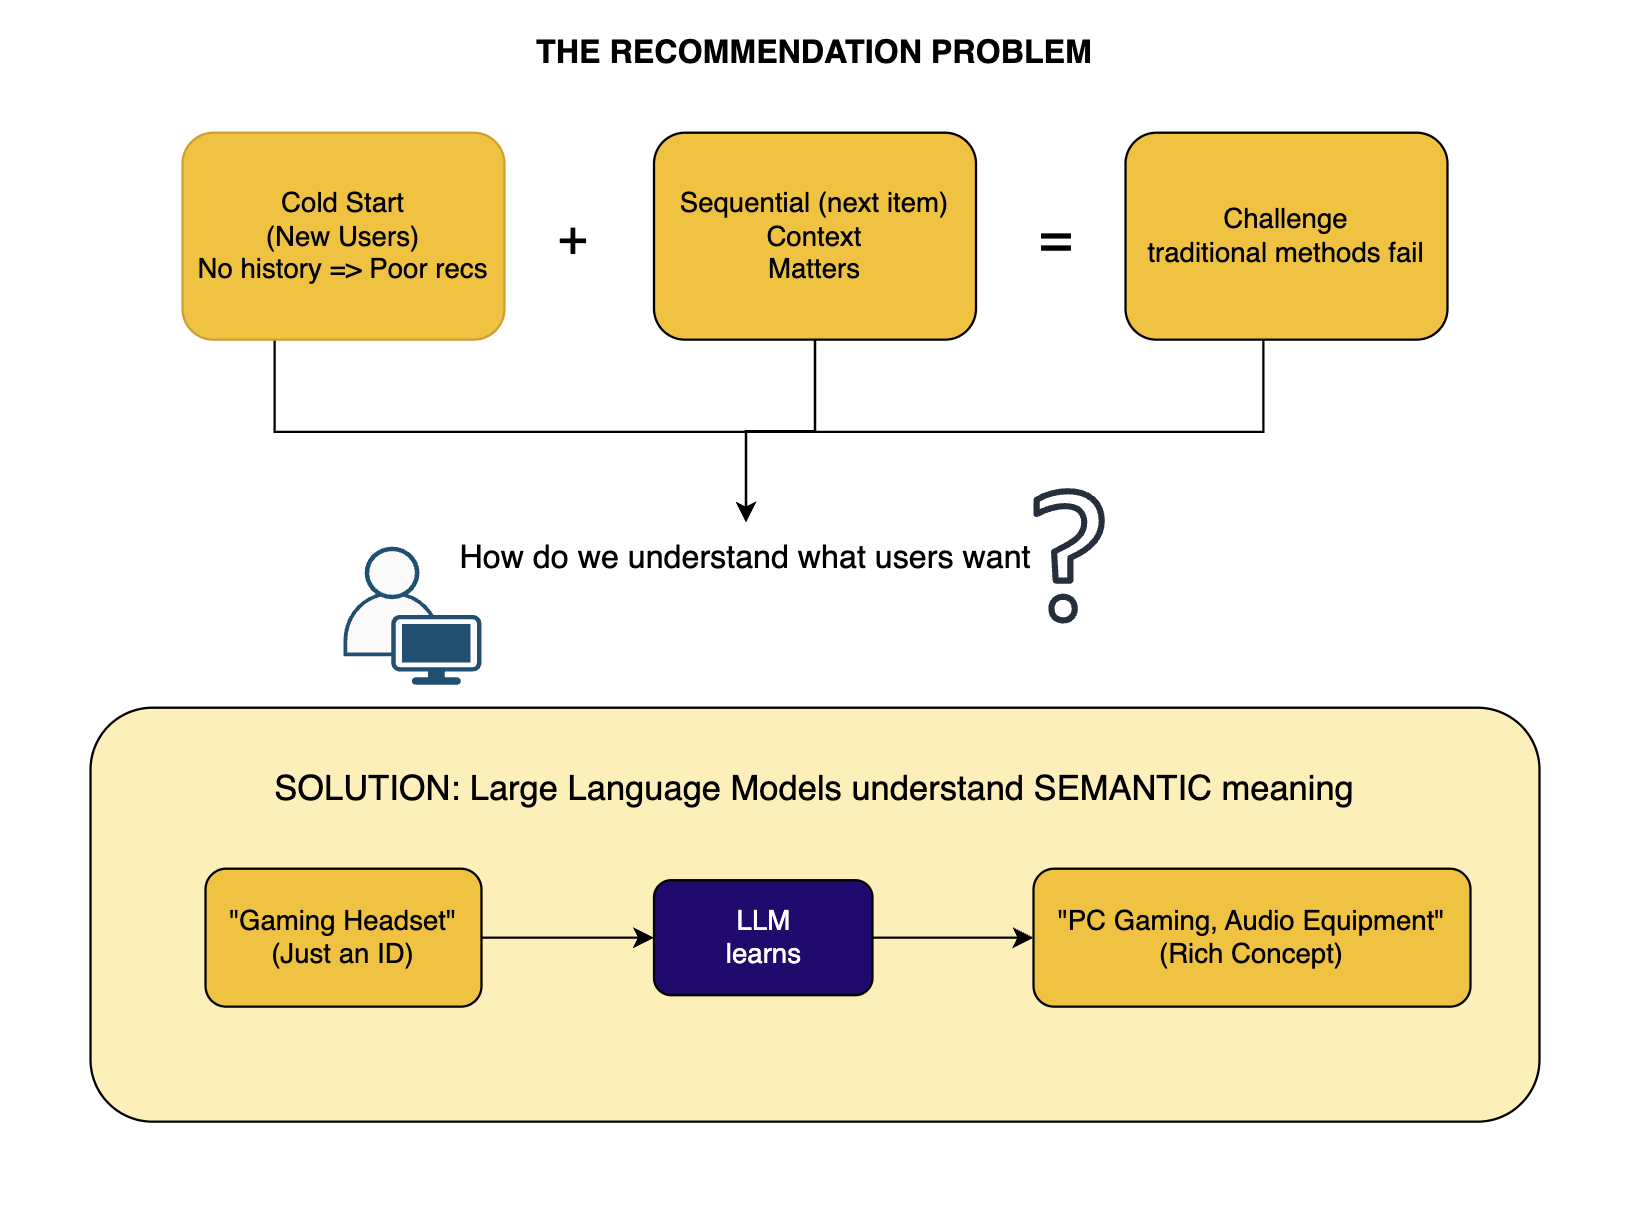
\includegraphics[width=\linewidth]{figures/Problem.png}
    \caption{Addressing the Cold Start and Sequential Constraints through Semantic Mapping.}
    \label{fig:performance_lift}
\end{figure}


\section{Literature Review}
The field of recommender systems changed significantly over the past years. Over time new systems have been introduced which can produce personalized recommendations considering not only user interactions but also the semantic meaning behind them. Recent advances in Large Language Models (LLMs) made a huge impact on utilizing user reviews to create accurate, diverse and meaningful recommendations \cite{b4}, \cite{b16}. Since recommender systems are used in various domains such as e-commerce, healthcare, media, etc, it is crucial for the companies to research and modernize their recommendation systems\cite{b19}. This section analyzes current approaches in the field, highlighting their strengths and weaknesses.


\subsection{Collaborative filtering }\label{AA}
Collaborative filtering (CF) is one of the most used methods in recommendation systems \cite{b17, b19}. The main idea of CF is to find a relationship between users and items relying on the fact that users who had similar behaviours towards the same items in the past, are going to perform similarly in future. For example, if Bob and John both liked the movie “Interstellar” in the past, and we know that Bob also liked the movie “Project Hail Mary”, then we can recommend it to John as well, because Bob and John have similar preferences. The main problem of the CF is that it struggles with cold-start and data sparsity problems \cite{b2, b19}.

We can categorize CF into two categories: memory-based and model-based \cite{b17}. Memory-based CF approaches consider user historical data to make predictions\cite{b16}. These systems utilize statistical methods to find similar items or users. For instance, many  memory-based rec systems use similarity metrics such as Cosine similarity or the Pearson Correlation Coefficient.

Memory-based methods excel in scenarios where the user base and item catalog are stable, and the system needs to be highly interpretable and simple to implement without requiring long offline training cycles \cite{b16}. However, when it comes to the large-scale datasets, they perform poorly, since they run longer and require more computational resources compared to smaller datasets.  The performance of memory-based methods drops significantly when data sparsity increases,  as it becomes difficult to find direct overlapping interactions between users\cite{b19}.

Model-based CF approach uses past user interactions to create a model which will then generate recommendations \cite{b1}. The main paradigm behind Model-based CF is Matrix Factorization \cite{b17}. Matrix factorization is a technique used for making big tables filled with items and users’ ratings smaller and easier to work with. Smaller tables capture hidden patterns (also called latent factors); for example, music genres. Then by multiplying those tables, we get the score of how much the user will like the new item they have not seen yet. One of the model-based CF approaches is Bayesian Personalized Ranking (BPR), which calculates the scores for particular items by prioritising the items that the user prefers \cite{b1}.

Model-based approaches perform well when uncovering non-trivial, abstract hidden patterns within sparse datasets \cite{b1,b11}. They can compute online recommendations fast because the heavy computational work is completed during offline training \cite{b17}. However, the performance drops when we have a user with limited or zero interaction data \cite{b2,b4,b11}.


\subsection{Modern Sequential Models}
Compared to the CF methods, sequential models consider the order of user behaviour to predict the user's next choice \cite{b2,b17, b19}. Thus, the sequence of the user’s past interactions plays an important role in these techniques \cite{b14}. SASRec (Self-Attentive Sequential Recommendation) considers a user's past interactions and decides which of them is more important for predicting the next item for the user \cite{b1,b14}. For example, SASRec remembers what books liked the user even months ago and uses that information to predict the next book that will interest the user. Previous work have shown that since SASRec considers the order of items in the user history, it handles the recommendation problem better than the CF approaches, however sequential recommender systems still lack the semantic context about the products \cite{b2,b4, b6, b11, b15}. 

\subsection{Integrating LLM into Rec Systems}
Using LLMs in the process of building a recommendation system can be highly beneficial since it solves the \textit{cold start} problem and helps not only to predict next items, but also tell why the user might like it  \cite{b11, b12, b18,b19}. The integration of LLMs has significantly advanced the current state-of-the-art by serving as intelligent semantic engines and user profile simulators that can deeply understand complex, human-like choice behavior \cite{b2,b5,b11,b14}. There are several methods to integrate LLMs into traditional recommendation systems and build a hybrid system \cite{b2,b4,b19, b10}.


\subsection{Hybrid Recommendation Systems}
The most effective recommendation systems are proven to be hybrid systems because they combine the best of both worlds by utilizing the behavioural signals of CF with the semantic capabilities of LLMs \cite{b1,b2, b4,b8, b19, b20}. 

One of the strategies of implementing hybrid systems is the embedding initialization, where LLM plays a role of a text reader and by processing the item metadata, it generates vectors, which can be used to initialize traditional models like SASRec, instead of using random weights and updating them later \cite{b2,b6}. Another method of integrating LLMs into recommendation systems is to give the LLM a role of a reranker\cite{b9,b20}. This approach includes giving the top \textit{N} item candidate list to LLM and asking it to rerank the items using in-context learning instructions \cite{b2, b13}. 

Previous studies highlight the creation of user personas as a great method of making next item predictions more accurate \cite{b3,b7}. When LLM is asked to create a user profile for a specific users and then rank the dataset items taking into account users’ profiles, the results of recommendation have proven to be outstanding \cite{b3,b11}. For example, Lyu et al. \cite{b3} demonstrated that injecting semantic profiling and advanced text prompting via their \textit{LLM-Rec} framework yielded a substantial performance lift, improving baseline recommendation accuracy (NDCG@10) by up to 33.1\% on sparse user histories. 


\subsection{Data Science Best Approaches and Preprocessing}\label{SCM}
The quality of models are highly dependent on the data that is being used \cite{b16, b17}. In the industrial context, experts use some filtering techniques to avoid noise and data sparsity \cite{b17}. For instance, $k$-core filtering is often applied to iteratively remove users and items with small amounts of interactions, guaranteeing that every remaining user and item has at least $k$ records in the dataset \cite{b17, b21}. Usually 5-core filtering is used for large-scale datasets and a limit of 4 interactions is used for smaller datasets. Moreover, datasets from various domains such as Beauty, Movies, Videogames are used for training the same set of models to ensure there is diversity in data domains and sizing and avoid biased or inaccurate results \cite{b2, b4}.

Applying $k$-core filtering presents distinct trade-offs that directly affect system optimization. The primary advantages include a massive reduction in data sparsity, faster model convergence, and the removal of accidental or "one-off" interaction noise that disrupts sequential pattern modeling \cite{b17,b21}. However, the core disadvantage is that it can introduce severe survival bias by filtering out long-tail items, effectively making the recommendation task artificially easier than it would be in a raw production environment \cite{b17}. 





\section{Methodology}
This study implemented a four-phase experimental design, starting with traditional approaches and moving on to more sophisticated Large Language Model (LLM) integration strategies for sequential recommendation.
\begin{table}[htbp]
\caption{Dataset Statistics}
\begin{center}
\resizebox{\columnwidth}{!}{% % This forces the table to match column width
\begin{tabular}{|l|c|c|c|c|}
\hline
\textbf{Dataset} & \textbf{Users} & \textbf{Items} & \textbf{Interactions} & \textbf{Avg Seq Length} \\
\hline
Industrial \& Scientific & 50,985 & 25,689 & 259,992 & 5.10 \\
\hline
Video Games & 94,762 & 25,482 & 530,300 & 5.60 \\
\hline
Cell Phones \& Accessories & 380,999 & 110,373 & 1,609,788 & 4.56 \\
\hline
\end{tabular}
}
\label{tab_stats}
\end{center}
\end{table}

\subsection{Datasets and Data Preparation}

Three Amazon product review datasets were selected from the UCSD Amazon Product Data repository: \textit{Industrial \& Scientific}, \textit{Video Games}, and \textit{Cell Phones \& Accessories} \cite{b21}. These categories were chosen for their domain diversity: 
\begin{itemize}
    \item \textbf{Industrial \& Scientific:} Includes technical, professional-grade equipment and laboratory supplies.
    \item \textbf{Video Games:} Contains highly descriptive and subjective product information.
    \item \textbf{Cell Phones \& Accessories:} Contains high-volume, sparse interactions with generic product titles.
\end{itemize}

The statistical characteristics of selected datasets, including user counts, item totals, interactions, and average sequence lengths are summarized in Table~\ref{tab_stats}. Average sequence lengths represent the average number of interactions per user in each dataset.


To improve the quality of the recommendation models and manage computational efficiency, this study utilized the pre-processed \textbf{5-core} datasets provided by the UCSD Amazon Product Data repository \cite{b21}. The 5-core method ensures a minimum density within the interaction matrix by requiring at least five associated interactions for every unique user and every unique item. 

In raw e-commerce data, a significant portion of users may only purchase a single item, and many products may receive only a single review. These rare occurrences create extreme data sparsity, where patterns are often lost to noise, preventing the system from learning meaningful behavioral signals. In this study, the 5-core datasets were specifically chosen for the following reasons:

\begin{itemize}
    \item \textbf{Reduced Noise:} By filtering out "one-off" or random interactions, the models focus on consistent user preferences over time. This leads to higher-quality training material based on steady choices rather than isolated incidents.
    \item \textbf{Sequential Depth:} Sequential models, such as \textbf{SASRec}, rely on historical context to predict future intent. A history of fewer than five items provides insufficient information for the transformer architecture to accurately model user patterns.
    \item \textbf{Computational Efficiency:} Removing low-information, sparse data points results in faster training cycles and lower memory requirements. The models converge more quickly when the "clutter" of irrelevant data is removed.
    \item \textbf{Reliable Evaluation:} Performance metrics such as \textbf{Hit@10} and \textbf{NDCG@10} are more statistically significant when users have enough history to make a "top ten" recommendation list relevant. This ensures that the evaluation reflects actual behavioral patterns rather than random chance.
\end{itemize}

The interactions in these datasets are chronologically ordered, making them ideal for sequential analysis. The study utilized the pre-split train/validation/test partitions provided by the repository (approximately 75\% train, 12.5\% validation, and 12.5\% test) \cite{b21}.

\subsection{First Phase: Traditional Baseline Models}

Four baseline approaches were implemented to establish performance benchmarks:

\begin{itemize}
    \item \textbf{TopPop (Statistical):} A non-personalized baseline that ranks items based on global popularity count \cite{b17}. It recommends the same items to all users regardless of individual histor \cite{b19}.
    \item \textbf{BPR (Matrix Factorization):} Bayesian Personalized Ranking utilizes matrix factorization to optimize a pairwise ranking loss \cite{b1,b17}. It maximizes the posterior probability that an observed interaction scores higher than an unobserved (negative) sample using gradient descent.
    \item \textbf{XGBoost (Feature-Based):} An ensemble of 100 decision trees trained to predict interaction probability. It incorporates multidimensional feature vectors, including user history length, global item popularity, category identifiers, price tiers, and social proof (review counts and star ratings) \cite{b16,b17}.
    \item \textbf{SASRec (Neural Sequential):} A self-attentive transformer-based model that captures long-term and short-term dependencies. SASRec served as the primary neural baseline due to its state-of-the-art performance and structural similarity to modern LLMs \cite{b1,b13,b14}.
\end{itemize}

For all models (except TopPop), a grid search with six trials was implemented to determine optimal hyperparameters.

\subsection{Second Phase: LLM Item Embeddings}

The second phase involved semantic enhancement using pre-computed embeddings. The \texttt{all-MiniLM-L6-v2} model was selected from the Sentence-Transformers library to generate 384-dimensional dense vector representations from concatenated item titles and descriptions. This model provides an optimal balance between quality and computational efficiency.

To integrate these with the SASRec baseline, dimensionality reduction was performed via a fully-connected projection layer ($384 \to 64$). A "freeze-then-fine-tune" strategy was employed: LLM embeddings were frozen for the first 5 epochs to allow SASRec to adapt its architecture to the semantic inputs before joint optimization occurred.

\subsection{Third Phase: LLM API Reranker}

Phase 3 evaluated the efficacy of LLMs in a reranking role. SASRec was first used to generate a list of the top 30 candidates. These candidates were then processed by \texttt{GPT-4o-mini} via asynchronous API calls. The prompt included the user’s interaction history, item metadata, and a chain-of-thought instruction to rank candidates based on semantic compatibility. To ensure economic feasibility, this phase was evaluated on a stratified sample of $N=2,000$ users.

\subsection{Forth Phase: LLM User Profile Reranker}

The final phase incorporated synthesized "user personas." \texttt{GPT-4o-mini} generated a one-sentence profile based on the user's history, which was then used as context to rerank the 30 candidates from the base model. Due to increased latency and API costs, this evaluation used a stratified sample of $N=250$ users, maintaining the interaction distribution of the full dataset.


\subsection{Tools and Frameworks}

The research was developed using \textbf{Python 3.10} and the following core libraries:
\begin{itemize}
    \item \textbf{PyTorch 2.0.1:} Neural network implementation.
    \item \textbf{Hugging Face Transformers 4.30.2 \& Sentence-Transformers 2.2.2:} LLM inference and embedding generation.
    \item \textbf{scikit-learn 1.2.2 \& XGBoost 1.7.5:} Baseline implementations and preprocessing.
    \item \textbf{pandas 2.0.2:} Data manipulation.
    \item \textbf{OpenAI Python SDK:} Asynchronous batching for GPT-4o-mini API calls.
\end{itemize}

\section{Results}

This section shows  the results from four phases of our research, pitting old-school methods against smart sequence learners and three separate ways of using large language models. A pattern shows up plainly that generating embeddings with LLM beat everything else by far, including modern LLM integrations using API calls and classic techniques. 

\subsection{Evaluation Metrics}

Two gold-standard metrics were used to assess recommendation quality:
\begin{itemize}
    \item \textbf{Hit@10 (H@10):} A binary indicator of whether the ground-truth item appears within the top 10 recommendations (measures recall).
    \item \textbf{NDCG@10:} Normalized Discounted Cumulative Gain, which weights correct predictions based on their specific position in the ranked list.
\end{itemize}




\begin{figure}[htbp]
    \centering
    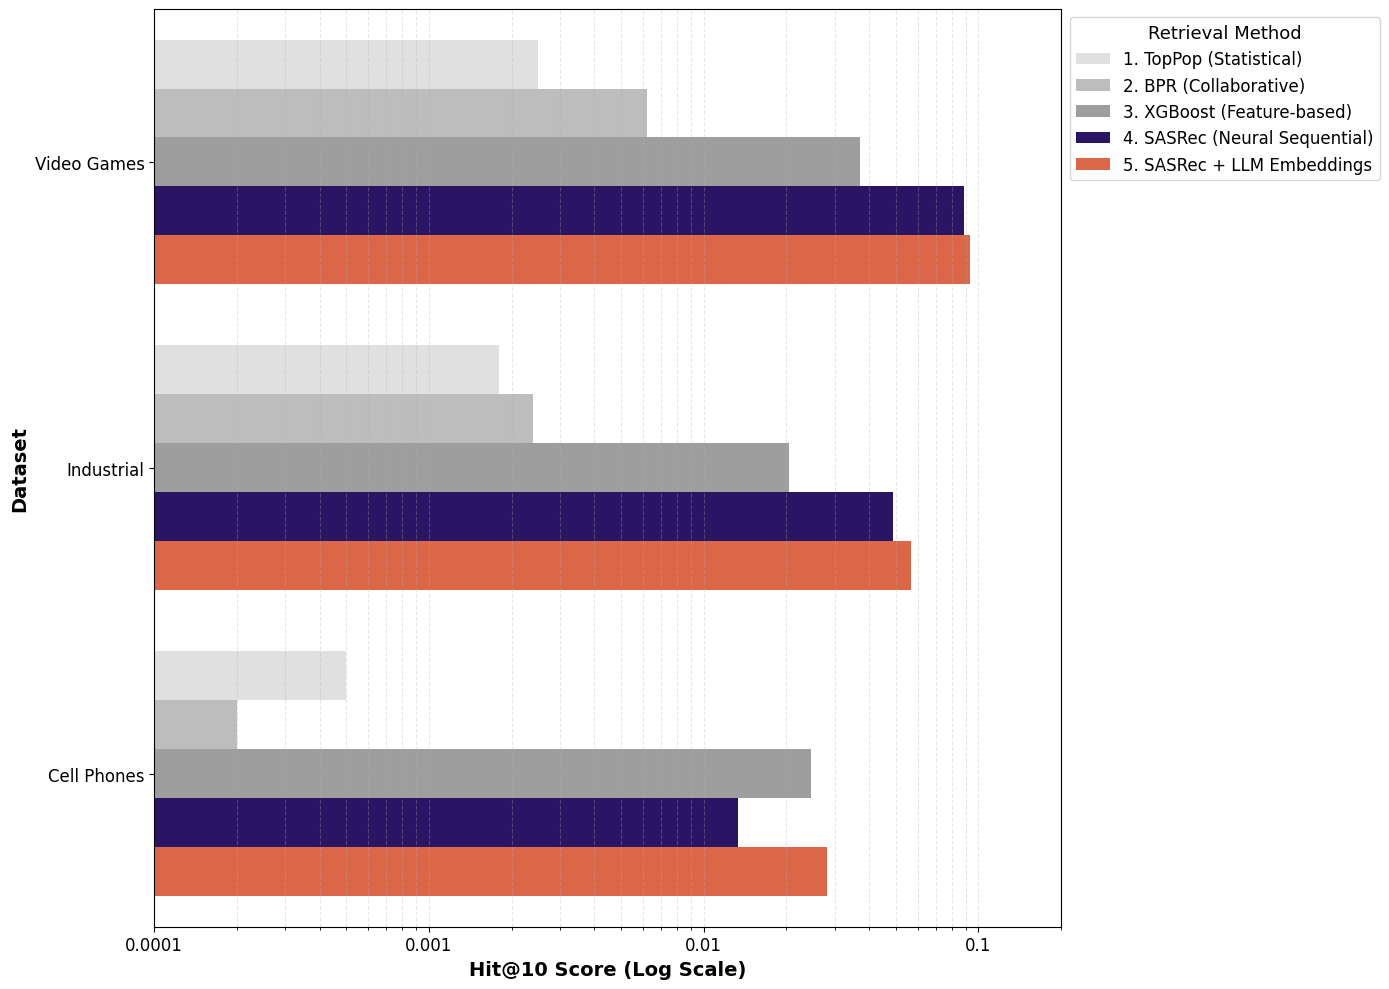
\includegraphics[width=\linewidth]{figures/graph1.png}
    \caption{Hit@10 Score across 5 recommendation approaches (Phase 1 and Phase 2)}
    \label{fig:hit_improvement}
\end{figure}

Figure~\ref{fig:hit_improvement} tracks Hit@10 across five recommendation approaches and three selected datasets, setting the floor and ceiling for what comes next. Old standards like TopPop and BPR barely register, scoring under 0.005 everywhere. Though TopPop just ranked items by overall fame, it missed what each person liked. Instead of combining signals, BPR tried splitting user tastes mathematically yet ignored order in choices. On the other hand, XGBoost used tailored inputs like cost level, type, and how often bought,  lifting results to 0.037 (Video Games), 0.020 (Industrial), 0.025 (Cell Phones). Even so, timing patterns in clicks stayed beyond reach. Moving forward, SASRec emerged as a neural starting point, hitting 0.088 (Video Games), 0.041 (Industrial), 0.038 (Cell Phones) on Hit@10. By focusing attention across past actions, its structure tracked sequences well, setting today’s benchmark for recommendations using only IDs. Still, seeing things just as random labels blocked deeper meaning. Figure~\ref{fig:hit_improvement} clearly shows that recommendations improve for all three datasets, when the SASRec model is initialized using embeddings generated with LLM. This is the starting point of LLM integration in our study.

\begin{figure}[htbp]
    \centering
    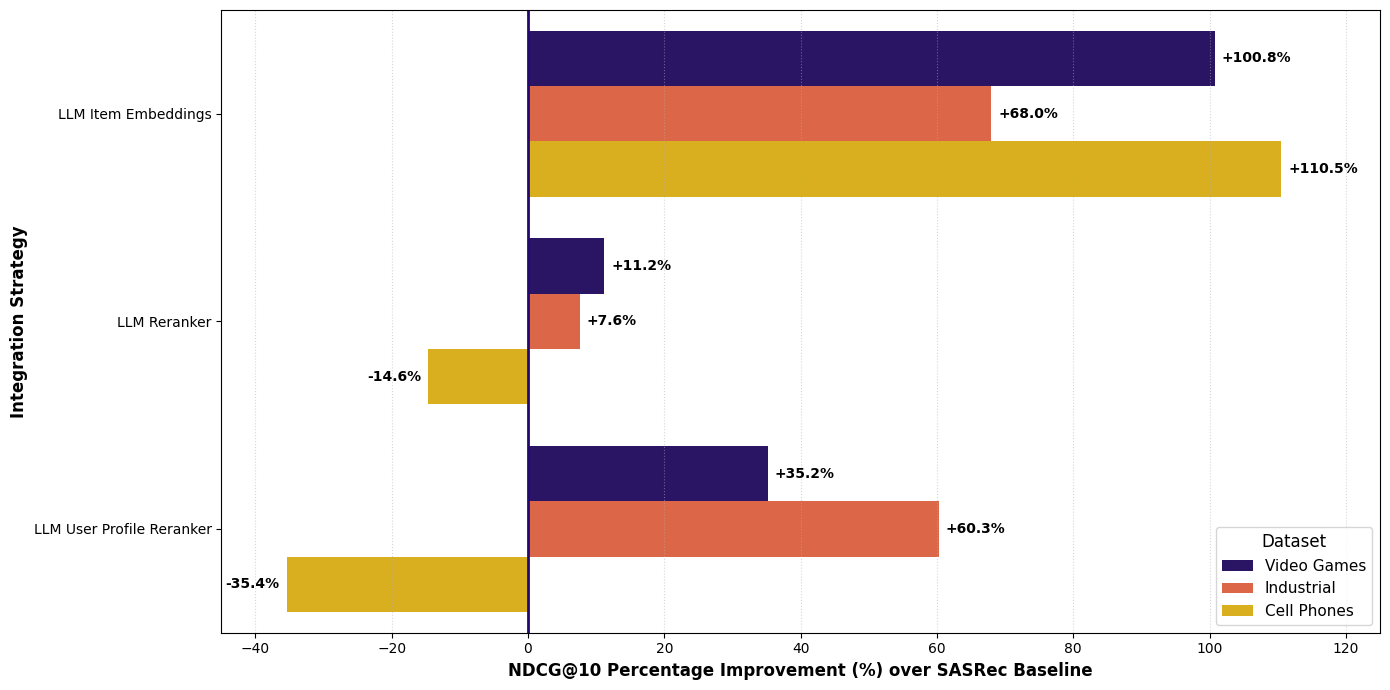
\includegraphics[width=\linewidth]{figures/graph2.png}
    \caption{NDCG@10 percentage improvement across all datasets for each LLM integration method.}
    \label{fig:ndcg_comparison}
\end{figure}

If we look at the NDCG@10 percentage improvement of LLM integration approaches over SASRec baseline in the Figure~\ref{fig:ndcg_comparison}, we can notice that tests show big improvements when slipping Large Language Models into recommendation steps, especially using LLM Item Embeddings, which worked best every single time. Jumping ahead, those embeddings pushed scores way up, more than doubling output on Video Games(+100.8\%) and Cell Phones(+110.5\%) against the older SASRec method. On the flip side, tossing in an LLM Reranker didn’t play out so smoothly, it helped Industrial and Video Games, but then backfired hard on Cell Phones, losing 14.6\%, even 35.4\%. 


Table~\ref{tab:ndcg_results} shows how well different methods using large language models work, measured by NDCG@10. These numbers come from tests on selected three datasets. As the sample size of experiments changes with each LLM integration method, SASRec baseline is evaluated for each method and dataset. This ensures that our comparisons are statistically accurate. 

Numbers show clear differences when comparing basic methods to those using large language models. Notably, SASRec paired with LLM embeddings pulls ahead every time. For instance, in case of the Video Games dataset NDCG@10 jumps from 0.0227 up to 0.0456. At the same moment. Considering Industrial \& Scientific data, another leap appears. There, NDCG@10 moves from 0.0125 to 0.0210, which is a solid 68\% jump compared to before.

Yet performance shifted by field. Though the LLM Profile Reranker hit an NDCG@10 of 0.0447 in Video Games , rising from a base score of 0.0331, it faltered badly with Cell Phones dataset. There, its NDCG@10 sank to 0.0073, dipping under the 0.0113 starting point. This hints that modeling user traits may grasp subtle needs, but seeding rankings through item embeddings still holds up best overall.

 
% --- NDCG Table ---
\begin{table*}[t]
\caption{NDCG@10 Performance Comparison Across LLM Integration Approaches}
\label{tab:ndcg_results}
\begin{center}
\begin{tabular}{|l|c|c|c|}
\hline
\textbf{Method} & \textbf{Video Games} & \textbf{Industrial \& Scientific} & \textbf{Cell Phones} \\
\hline
SASRec Baseline (Full) & 0.0227 & 0.0125 & 0.0133 \\
\hline
SASRec + LLM Embeddings (Full) & 0.0456 & 0.0210 & 0.0280 \\
\hline
SASRec Baseline (N=2000) & 0.0228 & 0.0140 & 0.0134 \\
\hline
SASRec + LLM Reranker (N=2000) & 0.0253 & 0.0151 & 0.0114 \\
\hline
SASRec Baseline (N=250) & 0.0331 & 0.0125 & 0.0113 \\
\hline
SASRec + LLM Profile Reranker (N=250) & 0.0447 & 0.0200 & 0.0073 \\
\hline
\end{tabular}
\end{center}
\end{table*}



\section{Analysis and Validation}
\subsection{Interpretation of Results}
Results show clear backing for the main hypothesis. With the integration of LLMs into sequence recommenders, outcomes get much better as mentioned in the Table~\ref{tab:ndcg_results}. Instead of just adding features, they used deep meaning from language models. Even though SASRec showed pretty good results and was a solid baseline, it still got beat by almost all LLM integration methods. 

What stands out is the jumps in NDCG@10 score for LLM embeddings across all datasets. This suggests that LLM-based embeddings improve how well results are ordered, not just whether correct items show up somewhere. These embeddings understand connections between items, so they arrange likely matches higher up the list. They don’t magically find more relevant things, instead, they sort what’s already there more intelligently. Since real users tend to look at recommendations starting at the very top and often stop early, the boost in rank accuracy matters far more than simply adding a few extra hits further down.

The API-driven reranking methods which were performed in Phases 3 and 4, show that using LLMs as rerankers in recommendation systems can improve the quality of recommendations. However, we can notice that these approaches are not the best choice for certain types of data. Phase 3 and 4 expose how unstable real-time LLM thinking can be inside rec systems. 

\textbf{Phase three LLM reranker performance review:} We notice 11.2\% improvement in NDCG@10 score in case of Video Games data and 7.6\% improvement on Industrial \& Scientific data. The results shift moving to the Cell Phones dataset, where things dropped by 14.6\%. Multiple reasons sit behind these outcomes.
Because descriptions matter a lot, how well the reranker works depends on what info it gets. In case of video games dataset, items names are packed with detail, like “Razer DeathAdder Elite Gaming Mouse, 16000 DPI Optical Sensor,” giving the model plenty to go on. Technical specs show up in industrial items too, just in a different way. But in the case of phone accessories, the descriptions are not detailed. Titles such as “iPhone14 Case” pop up often, offering almost nothing useful to work with.
Even if the reranker works well, its impact depends heavily on what comes before. Starting from SASRec’s best 30 suggestions means working within tight boundaries. If those initial picks are strong, reshuffling them changes little. But when early results miss the mark, fixing gaps becomes impossible. That’s because new options never get added, only positions shift. So performance hinges on earlier stages doing their job right.

\textbf{Phase four LLM user profile reranker performance review:} the user profile reranker showed great results on  Video Games showing the NDCG@10  improvement of 35.2\% compared to the SASRec baseline and a spike of 60.3\% gain in Industrial \& Scientific data. However, we notice a sudden decrease of  35.4\% in performance for Cell Phones dataset. 

The results suggest that generating user profiles and incorporating them into the recommendation systems can certainly help to increase the quality of recommendation systems, however this approach is not suitable for the sparse data such as the selectd Cell Phones dataset. The wrong details might slip into a user's profile during creation. When systems guess traits from past actions, mistakes happen. Buying phone cases once could label someone as caring about trends instead of safety. This mix-up pushes the system to favor flashy options over useful ones. Looks get priority even when they miss the point.

Wrong details in a profile grow worse as they move through the ranking steps. When the initial character description is off, every following choice gets pulled further wrong. The simpler third phase reranker skips extra stages, so mistakes have less room to build up. Therefore the results of recommendations for the Cell phones dataset are worse for the fourth phase compared to the third phase.

Sample size for Phase 4 testing was 250 because generating profiles and reordering results took too much computing power. Even though the stratified sampling was used, not using the full dataset can lead to not capturing a broader range of actions means real-world patterns might be missed entirely. 

\subsection{Comparison with Baseline Methods}
Older methods like TopPop, BPR, and XGBoost set reference points showing how well newer models do. Though popular items often get noticed, TopPop’s one-size-fits-all ranking scored under 0.005 on Hit@10 every time, proving it misses personal tastes in big collections. Even BPR, which learns hidden patterns to tailor results, stumbled because it ignores order in user behavior, so its outcomes stayed weak too.

Starting strong, XGBoost stood out among classic models by using carefully built features, scoring 0.037 on Video Games, then 0.020 for Industrial supplies, along with 0.025 in Cell Phones when measuring Hit@10. Features like how often an item sold, what group it belonged to, pricing level, plus feedback from buyers, such as rating averages and total reviews, helped push its results higher. Still, patterns over time in how users acted were missed entirely by this method. That gap showed clearly once compared to SASRec, a model tuned to such shifts, hitting 0.088 in case of the Video Games, jumping to 0.041 for  Industrial supplies, also reaching 0.038 across Cell phones data.

Starting fresh, SASRec set a solid base using attention mechanisms on sequences, leading today's item-ID recommendations. Yet viewing products just as labels blocked deeper meaning capture. Into that gap stepped LLM embeddings, sliding rich semantic context straight into the framework, performance jumped up to 110.5\% in NDCG@10 without slowing things down.

\subsection{Validation Techniques}

Checks happen in different ways to back up results, making sure they hold true across situations
Stratified sampling was used to face the computational challenges. The sample kept how often each history length showed up in the full dataset. In phase three, two thousand entries were pulled. Because generating user profiles before reranking is computationally heavy, only two hundred fifty made it into phase four. By keeping the distribution of the sample the same as the original dataset, we ensured that our experiments are statistically valid and we tried to give the models as equal opportunities to succeed at recommending as possible. 

One way to check each LLM method was by matching it directly with its own SASRec version using identical groups of users. Because both systems saw the exact same people, any change in results likely came from how the LLM was added, not random differences in data selection.
The datasets were partitioned using a chronological 75/12.5/12.5 train-validation-test split strategy. This split allocation ensures that 75\% of the historical interaction sequences are dedicated to model training and convergence, while maintaining perfectly symmetrical subsets for evaluation. Consequently, the 12.5\% validation set is utilized for iterative hyperparameter tuning via grid search, leaving an equally robust 12.5\% test set completely untouched for final, unbiased performance evaluation.

\subsection{Limitations}

Despite the performance gains observed, several limitations were encountered during this research:

\begin{itemize}
    \item \textbf{Computational and Cost Constraints:} Due to the financial and computational overhead associated with large-scale API inference, the reranking approaches were evaluated on stratified subsets ($N=2,000$ for Phase 3 and $N=250$ for Phase 4). While stratified sampling was utilized to maintain distributional representativeness, the restricted sample size in the final phase may limit statistical power and increase the variance of the reported metrics.
    \item \textbf{Metadata Quality and Noise:} some of the LLM integration approaches(Phase 3,4) rely heavily on the metadata of items. For instance, in categories like \textit{Cell Phones}, where titles are often technical or generic, the LLM’s ability to find meaningful semantic links is diminished compared to categories with rich, descriptive content like \textit{Video Games}.
\end{itemize}


\section{Discussion and Conclusion}

The findings of this study strongly support the hypothesis that LLMs could significantly improve the performance of recommendation systems by incorporating semantic understanding, nearly doubling NDCG@10 across multiple product categories. However, this study revealed that despite model complexity, some LLM approaches like user profile reranking can underperform compared to simpler integration strategies such as item embedding generation. These results validate that practitioners can achieve significant improvements, without expensive GPU infrastructure or API subscriptions, making semantic understanding accessible to any organization with commodity CPU hardware.


\section*{Acknowledgment}

The authors would like to thank the UCSD Amazon Product Data repository for providing the datasets used in this study.

Additionally, we thank the academic community for the foundational research in sequential recommendation and large language models that inspired and informed this study.


\bibliographystyle{IEEEtran} 
\bibliography{references}


\end{document}
